% Base sur la VO 0.11.9
% Relecture technique: 
% Relecture syntaxique: 

\part{Mise en place de la partie}

Pour jouer à \emph{BF : Le 9\ieme Âge}, il y a plusieurs étapes à suivre afin de mettre le jeu en place. La première étape est de trouver un adversaire et de vous mettre d'accord sur la taille de la partie. Les joueurs peuvent ensuite se dévoiler leurs listes d'armée et commencer à installer le champ de bataille. Puis ils déterminent le type de déploiement, le choix des objectifs secondaires du jeu, les zones de déploiement et ils génèrent les sorts de leurs sorciers. La dernière étape consiste à passer à ce qu'on appelle le déploiement.

\section{Étapes de la préparation}

La table \ref{table/etapes_preparation} résume les différents préparatifs.

\begin{table}[!htbp]
\centering
\begin{tabular}{c|l}
\textbf{1} & Décidez de la taille de la partie. \tabularnewline
\textbf{2} & Montrez-vous vos listes d'armée. \tabularnewline
\textbf{3} & Installez les décors du champ de bataille. \tabularnewline
\textbf{4} & Déterminez le type de déploiement. \tabularnewline
\textbf{5} & Choisissez les objectifs secondaires. \tabularnewline
\textbf{6} & Déterminez les zones de déploiement. \tabularnewline
\textbf{7} & Générez les sorts. \tabularnewline
\textbf{8} & Déployez-vous. \tabularnewline
\end{tabular}
\caption{\label{table/etapes_preparation}Préparatifs préalables à une partie.}
\end{table}

\section{Taille de la partie}

La première étape d'une partie de \emph{BF : Le 9\ieme Âge} est bien entendu de décider de la taille de la bataille, c'est-à-dire du nombre de points dont chaque adversaire dispose pour construire son armée. Deux armées qui se font face devraient toujours faire la même taille. Mettez-vous d'accord sur un nombre de points qui vous convient.

\section{Dévoiler les listes}

L'étape suivante est d'échanger les listes d'armée ainsi que toute information pertinente à propos de la partie à venir. Les joueurs peuvent aussi choisir de garder quelques informations secrètes, et de ne les révéler qu'au fur et à mesure de la partie, comme expliqué dans le paragraphe \ref{liste_cachee}.

\section{Placer les décors}

La partie se joue sur un champ de bataille de 48{\pouce} par 72{\pouce} soit environ 1,20 {\meter} par 1,80 {\meter} pour les tailles d'armée standard (entre 1500 et 4000 points). Pour de plus petites batailles, au format \emph{Patrouilles}, nous recommandons une table d'environ 90 {\centi\meter} par 1,20 {\meter} (36{\pouce} par 48{\pouce}), et pour les plus grandes parties, au format \emph{Grandes Armées}, le champ de bataille sera d'autant plus grand que les armées le seront. Bien que certaines parties puissent être jouées sur un champ de bataille complètement découvert, on y place habituellement quelques décors.

Les deux joueurs peuvent tout à fait s'entendre sur la taille, le type et le nombre de décors à placer, ainsi que sur leurs positions. Si vous n'arrivez pas à vous mettre d'accord, utilisez les règles ci-dessous pour mettre en place le champ de bataille.

\begin{itemize}[label={-}]
\item Divisez le plateau de jeu en sections de 24{\pouce} par 24{\pouce}, soit environ 60 {\centi\meter} par 60 {\centi\meter} \newrule{(Si la table fait 36{\pouce} par 48{\pouce}, prendre des sections de 18{\pouce} par 24{\pouce}, soit environ 45 {\centi\meter} par 60 {\centi\meter})}.

\item Placez les décors suivants au centre de sections désignées aléatoirement, avec un décor au plus dans chaque section : un \emph{Bâtiment} ou un \emph{Terrain Infranchissable} (tirez au hasard), une \emph{Colline} et une \emph{Forêt}. Déplacez ensuite chaque décor de 2D6{\pouce} dans une direction aléatoire.

\item Puis ajoutez 2D3 décors \newrule{(1D3 si la table fait 36{\pouce} par 48{\pouce})}, en suivant les règles ci-dessus pour leur positionnement. Lancez 1D6 pour déterminer le type de chaque décor additionnel :
\begin{enumerate}
\item Colline
\item Forêt
\item Champ
\item Eau peu profonde
\item Mur
\item Ruines
\end{enumerate}

\item Tous les décors doivent être placés au moins à 6{\pouce} les uns des autres. Bougez-les aussi peu que possible de leur position initiale pour satisfaire à cette condition. Si cela n'est pas possible, retirez le décor qui pose problème.
\item Les tailles de décors recommandées sont entre 6{\pouce} par 8{\pouce} (15x20 cm) et 6{\pouce} par 10{\pouce} (15x25 cm), excepté pour les \emph{Murs}, pour lesquels on conseille 1{\pouce} par 10{\pouce} (2,5x25 cm).
\end{itemize}

\section[Type de déploiement]{\nouveau{Type de déploiement}}

Les deux joueurs peuvent se mettre d'accord sur le type de déploiement, ou vous pouvez le tirer au hasard en lançant 1D6 :
\begin{itemize}[label={-}]
\item \emph{1 à 3}. Classique. La table est divisée en deux moitiés égales par une ligne centrale, dans le sens de la longueur. Le déploiement se fait à plus de 12{\pouce} de part et d'autre de cette ligne. 
\item \emph{4 à 5}. Diagonale. La table est divisée en deux moitiés par une diagonale de la table. Le joueur choisissant sa zone de déploiement décide laquelle utiliser. Le déploiement se fait à plus de \nouveau{9{\pouce}} de part et d'autre de cette ligne. 
\item \emph{6}. \nouveau{Attaque de flanc}. La table est divisée en deux moitiés égales par une ligne centrale, dans le sens de la longueur. Le joueur choisissant sa zone de déploiement décide s'il veut être l'attaquant ou le défenseur. L'attaquant peut se déployer à plus de 9{\pouce} de la ligne centrale à plus du quart des bords courts de la table (18{\pouce} sur une table de 72{\pouce} de long), et à plus de 15{\pouce} de la ligne médiane aux deux autres endroits (près des bords courts). Le défenseur fait le contraire, les limites de 9{\pouce} et 15{\pouce} sont inversées.
\end{itemize}

La figure \ref{figure/deploiement} illustre ces trois types de déploiement.

\begin{figure}[!htbp]
\centering

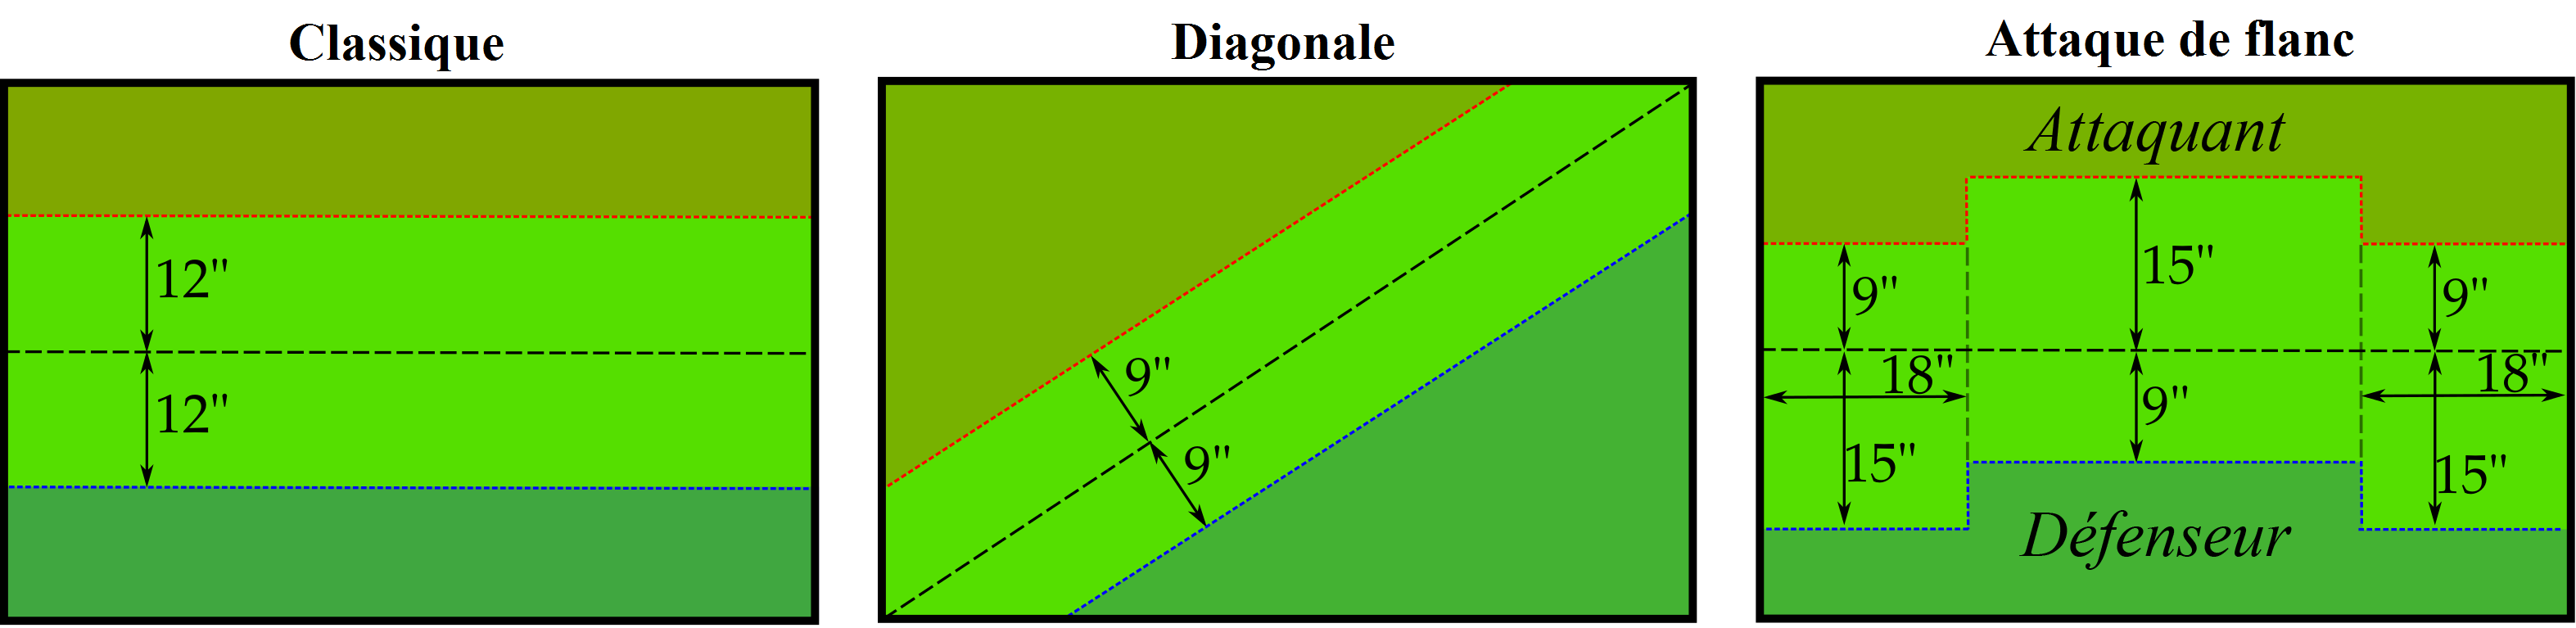
\includegraphics[width=14cm]{deploiement.png}
\caption{Illustration des trois types de déploiement.}
\label{figure/deploiement}
\end{figure}

\section[Objectifs secondaires]{\nouveau{Objectifs secondaires}}

Les deux joueurs peuvent se mettre d'accord sur l'objectif secondaire, ou vous pouvez le déterminer aléatoirement en lançant 1D6 : 
\begin{itemize}[label={-}]
\item \emph{\result{1} ou \result{2}}. Tenez la ligne. \emph{Tenez et défendez le centre du champ de bataille.} Placez un marqueur sur le centre du champ de bataille si nécessaire.
\item \emph{\result{3} ou \result{4}}. Percée. \emph{Envahissez le territoire ennemi.}
\item \emph{\result{5}}. \newrule{Capturez les étendards. \emph{Des cibles de valeur doivent être annihilées.} Après les mouvements d'avant-garde, avant de déterminer qui aura le premier tour de jeu, les deux joueurs doivent désigner ouvertement 3 porte-étendards ennemis (à l'exception du porteur de la grande bannière), en commençant par le joueur qui a terminé son déploiement en premier. Si un joueur possède moins de 3 porte-étendards dans son armée, son adversaire désignera tous ses porteurs d'étendards. Les porte-étendards des \emph{Troupes Légères} ne peuvent pas être désignés, mais ceux qui n'ont pas été encore déployés (comme pour les unités en \emph{Embuscade}) peuvent l'être.}
\item \emph{\result{6}}. Sécurisez cette zone. \emph{Des ressources cruciales ne doivent pas tomber entre les mains de l'ennemi.} Après avoir choisi les zones de déploiement, chaque joueur place un marqueur sur le champ de bataille, en commençant par celui qui a choisi sa zone de déploiement. Ces marqueurs doivent être positionnés à plus de 12{\pouce} de la zone de déploiement du joueur qui le place, et à plus de 24{\pouce} l’un de l’autre.
\end{itemize}

Voir la section \ref{condition_victoire} (page \pageref{condition_victoire}) sur les conditions de victoire pour les règles concernant les objectifs secondaires.

\section{Zones de déploiement}

Tirez au hasard afin de déterminer les zones de déploiement. Par exemple, un joueur peut lancer 1D6. Sur 4+, celui qui a lancé le dé choisit son côté de déploiement. Il choisit aussi la diagonale à utiliser pour le déploiement diagonal et qui joue le rôle de l'attaquant et du défenseur dans le cas de l'attaque de flanc.

\section{Générer les sorts}
\label{generation_sorts}

Chaque joueur génère les sorts pour tous ses \emph{Sorciers}, \nouveau{en commençant par le joueur qui a choisi sa zone de déploiement.} Pour cela, sélectionnez un \emph{Sorcier} et consultez la \emph{Discipline Magique} choisie (qui doit être inscrite sur la liste d'armée). Toutes les \emph{Disciplines Magiques} peuvent être trouvées dans \emph{Batailles Fantastiques : Le 9\ieme Âge, Disciplines Magiques}. Les sorts sont numérotés de 0 à 6. Lancez autant de D6 que de sorts que le \emph{Sorcier} possède (normalement en nombre égal à son niveau de magie) pour voir à quels sorts le \emph{Sorcier} a accès pour cette bataille. Si un '1' est obtenu, le \emph{Sorcier} connaît le sort numéro 1, et ainsi de suite. Si un sort est obtenu deux fois (les dés donnent un double, ou bien un autre \emph{Sorcier} dans la même armée a déjà choisi le sort), le \emph{Sorcier} doit remplacer le sort en double par un autre sort de la même \emph{Discipline Magique} de son choix qui n'a pas encore été choisi. Deux \emph{Sorciers} de la même armée ne peuvent pas choisir le même sort, et aucun \emph{Sorcier} ne peut connaître un sort plus d'une fois. S'il est impossible de remplacer un sort en double par un sort disponible, le sort est perdu. De plus, le \emph{Sorcier} peut échanger un de ses sorts pour le sort primaire de sa \emph{Discipline Magique} (numéroté 0). Le sort primaire peut être choisi même si d'autres \emph{Sorciers} l'ont déjà sélectionné.

Les sorts qui ne sont pas générés en suivant ces règles sont ignorés pour la duplication des sorts, comme les \emph{Sorciers} qui ont des sorts prédéterminés ou tous les objets de sorts. De tels sorts peuvent ainsi être présents plus d'une fois dans la même armée.
